\section{Trends and distributions in ACU Literature}\label{sec:appendix_trends}

Based on the information that we collect from the reviewed literature (see details in \Cref{sec:appendix_tables}), we further analyze the statistics of important topics related to ACU. Specifically, we identify the frequencies, trends, and distributions to highlight key insights.
An interactive versions of the plots presented below are available on our project page at \url{https://sagerpascal.github.io/agents-for-computer-use}.


\begin{figure}[htbp]
    \centering
    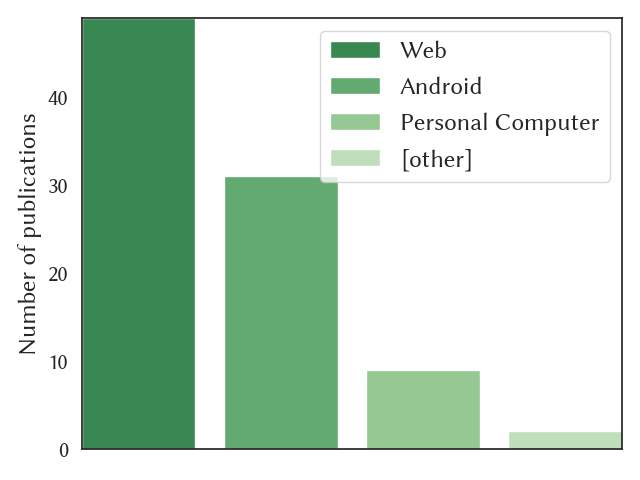
\includegraphics[width=0.48\linewidth]{figures/data/domain_dist.png}
    \caption{Number of ACU publications across domains, showing a strong preference for web-based platforms, followed by Android and personal computers.}
    \Description{A plot showing the number of agent publications with green bars. $49$ ACUs target web-based platforms, $31$ target Android, $9$ target personal computers, and $2$ target other domains. The figure highlights the concentration of research efforts on web and Android environments.}
    \label{fig:domain-dist}
\end{figure}

\begin{figure}[htbp]
    \centering
    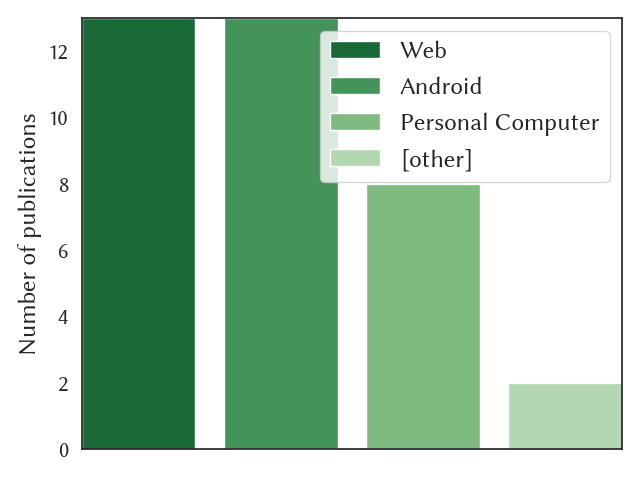
\includegraphics[width=0.48\linewidth]{figures/data/dataset_domain_dist.png}
    \caption{Dataset counts across domains. The distribution of datasets shows that most datasets analyzed in this study are from the Web and Android domains.}
    \Description{A plot showing the number of datasets publications with green bars. There are 13 datasets focusing on Web, $13$ datasets focusing on Android, $8$ datasets focusing on personal computers, and $2$ datasets focusing on other domains. This illustrates the alignment between dataset availability and research focus in ACU studies.}
    \label{fig:dataset-domain-dist}
\end{figure}

\begin{figure}[htbp]
    \centering
    \begin{minipage}[t]{0.48\textwidth}
        \centering
        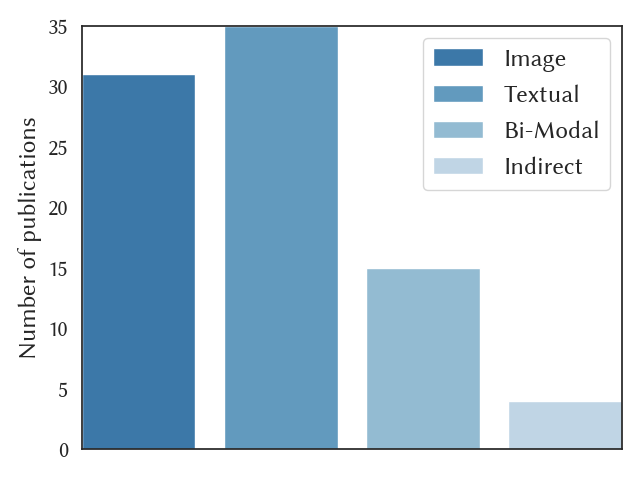
\includegraphics[width=\linewidth]{figures/data/observation_space_dist.png}
    \end{minipage}
    \hfill
    \begin{minipage}[t]{0.48\textwidth}
        \centering
        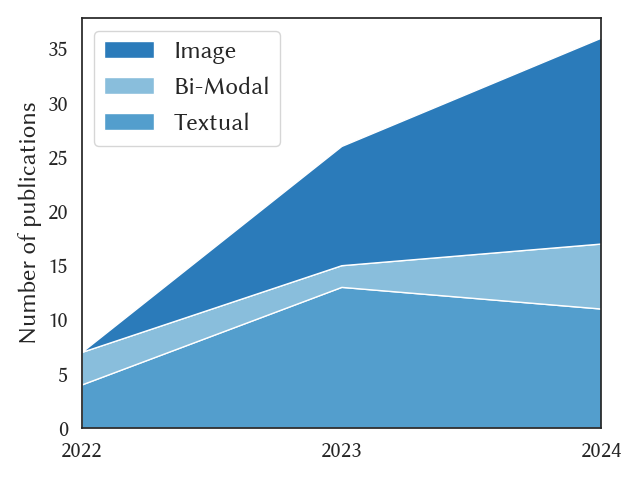
\includegraphics[width=\linewidth]{figures/data/observation_space_trend.png}
    \end{minipage}
    \caption{(left) Frequencies over all years and (right) trends as a stacked area plot of publications of observation spaces. It shows rapid growth in image and bi-modal.}
    \Description{Two plots, both showing the number of publications for different observation spaces. The left subplot is a bar plot, showing that $35$ ACUs use textual observations, $31$ ACUs use image observations, $15$ ACUs use bi-modal observations, and $4$ ACUs use indirect observations. The right subplot is a stacked area plot illustrating trends in the number of publications using each modality from 2022 to 2024.  Image-based observation usage shows a pronounced increase over time, from $0$ in 2022 to $12$ in 2023 and $19$ in 2024. In contrast, textual and bi-modal modalities remain relatively stable, with textual at $3$, $10$, and $8$ publications, and bi-modal at $1$, $1$, and $2$ publications across the three years, respectively.}
    \label{fig:observation-space-trend}
\end{figure}

\begin{figure}[htbp]
    \centering
    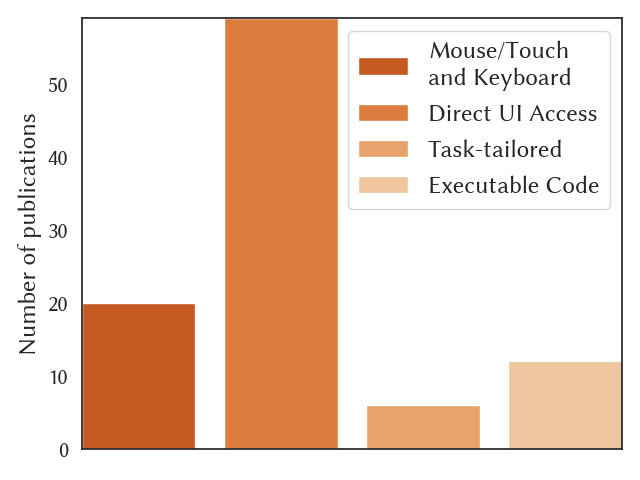
\includegraphics[width=0.48\linewidth]{figures/data/action_space_dist.png}
    \caption{Frequencies of action spaces. Agents with multiple action types are counted once.}
    \Description{A bar plot showing the number of ACU publications per action space. The most common action type is direct user interface access ($59$ ACUs), followed by mouse/touch and keyboard actions ($20$ ACUs). Executable code ($12$ ACUs) and task-tailored actions ($6$ ACUs) are less frequent.}
    \label{fig:action-space-dist}
\end{figure}

\begin{figure}[htbp]
    \centering
    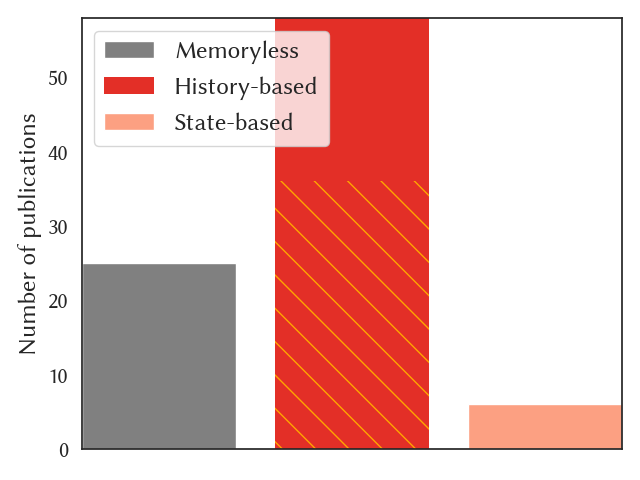
\includegraphics[width=0.48\linewidth]{figures/data/policy_dist_with_hatches.png}
    \caption{Frequencies of policy types. Orange strips indicate agents that only track past actions.}
    \Description{A bar plot showing the number of ACU publications for different policy types. There are $58$ ACUs using history-based policies (from which $36$ only track past actions), $25$ ACUs use memoryless policies, and $6$ ACUs use state-based policies.}
    \label{fig:policy-dist}
\end{figure}

\begin{figure}[htbp]
    \centering
    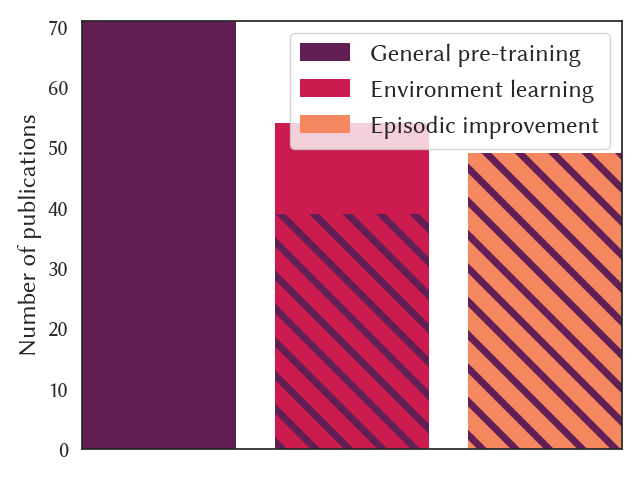
\includegraphics[width=0.48\linewidth]{figures/data/learning_strategy_dist.png}
    \caption{Frequencies of learning strategies. Purple stripes indicate initial pre-training.}
    \Description{A bar plot showing the number of ACU publications for different learning strategies. $70$ ACUs use general pre-training, $53$ ACUs use environment learning (from which $38$ are pre-trained), and $49$ ACUs use episodic improvement (from which all are pre-trained).}
    \label{fig:learning-strategy-dist}
\end{figure}

\begin{figure}[htbp]
    \centering
    \begin{minipage}[t]{0.48\textwidth}
        \centering
        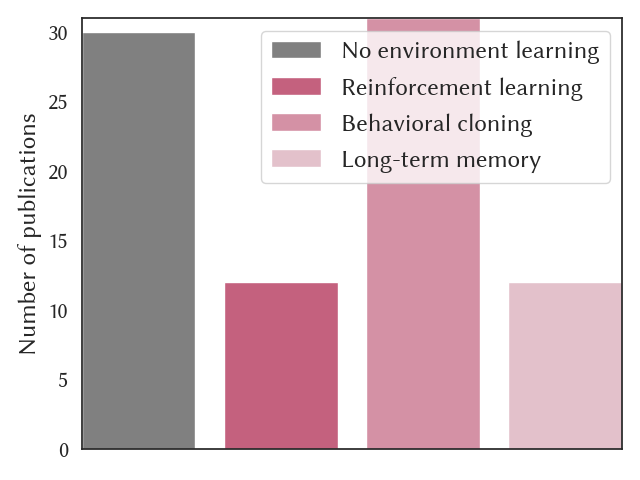
\includegraphics[width=1.0\linewidth]{figures/data/environment_adaption_dist.png}
    \end{minipage}%
    \hfill
    \begin{minipage}[t]{0.48\textwidth}
        \centering
        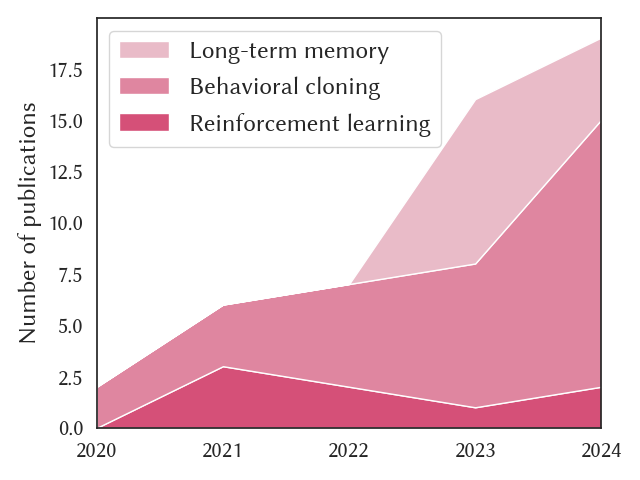
\includegraphics[width=1.0\linewidth]{figures/data/environment_adaption_trend.png}
    \end{minipage}
    \caption{
    (Left) Frequencies over all years and (right) usage trends as staked area plot of environment learning strategies over the last 5 years. It shows that behavioral cloning is the most adopted method.
    }
    \Description{Two plots, both showing the number of publications for different environment learning strategies. The left plot is a bar plot, showing that 31 ACUs use behavior cloning, 30 ACUs use no environment learning, 12 ACUs use reinforcement learning, and 12 ACUs use long-term memory.
    The right panel is a stacked area plot showing yearly trends from 2020 to 2024. Behavioral cloning has increased steadily, from $2$ publications in 2020, to $3$ in 2021, to $5$ in 2022, to $7$ in 2023, and to $12$ in 2024.
    The number of reinforcement learning publications is rather constant over time ($0$ publications in 2020, $3$ in 2021, $2$ in 2022, $1$ in 2023, and $2$ in 2024).
    Long-term memory appears for the first time in 2023 and is directly used by $8$ ACUs, while $4$ agents used it in 2024.
    }
    \label{fig:environment-adaption-dist}
\end{figure}
